%\documentclass[headsepline,titlepage,twoside,12pt]{report}
\documentclass[headsepline,titlepage,twoside,12pt]{scrreprt}
\usepackage[utf8]{inputenc}
\usepackage[english]{babel}
\usepackage{fontspec}
\newfontfeature{Microtype}{protrusion=default;expansion=default;}%
%\setmainfont{texgyrepagella-regular.otf}[%
%  Microtype,
%  Ligatures = TeX,
%  BoldFont = texgyrepagella-bold.otf,
%  ItalicFont = texgyrepagella-italic.otf,
%  BoldItalicFont = texgyrepagella-bolditalic.otf,
%]%
%\setmainfont{texgyreheros-regular.otf}[
%    Microtype,
%    Ligatures = TeX,
%    BoldFont = texgyreheros-bold.otf,
%    ItalicFont = texgyreheros-italic.otf,
%    BoldItalicFont = texgyreheros-bolditalic.otf,
%]
%\usepackage{helvet} % helvetica sans serif font
%\setmainfont[Ligatures=TeX]{TeX Gyre Heros}
\usepackage[a4paper,top=4cm,bottom=3cm,left=4cm,right=3cm]{geometry}
\usepackage{graphicx}
\usepackage[onehalfspacing]{setspace}
\usepackage{tabularx}
\usepackage{tabulary}
\usepackage{booktabs}
\usepackage{amsmath}
\usepackage{csquotes}
\usepackage{microtype}% optional, looks better but can be commented out if it causes errors e.g. on MiKTeX
\usepackage{natbib}
\usepackage{hyperref}
\PassOptionsToPackage{pdfborder={0 0 0}}{hyperref} %Für finale gedruckte Ausgabe, ohne hervorgehobene Links
\usepackage{cleveref}
\usepackage{rotating}
\usepackage{xcolor}
%\renewcommand{\familydefault}{\sfdefault} % sans serif for everything except math
%\usepackage{tgheros} % Load the tgheros package for Helvetica-like font
\definecolor{nfdiblue}{HTML}{0abaf0}
%\usepackage{sectsty}
%\sectionfont{\color{nfdiblue}\Large\bfseries}
%\chapterfont{\color{nfdiblue}\Large\bfseries}
\addtokomafont{chapter}{\color{nfdiblue}}
\addtokomafont{title}{\color{nfdiblue}}

\newcommand{\thedate}{\today}
\newcommand{\theauthor}{Jane Doe}
\newcommand{\theeditor}{Jon Doe}
\newcommand{\thecontributors}{Jumbo Doe}

\author{\theauthor}
\date{\thedate}
\title{Title}
\titlehead{\vspace{-1.9cm}\hfill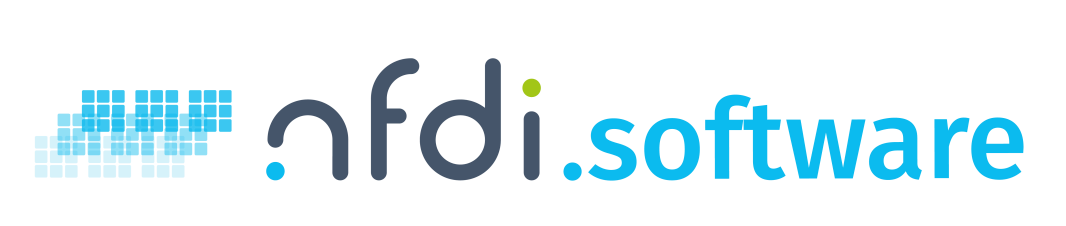
\includegraphics[width=13.5cm]{img/nfdi-software.png}\vspace{3cm}}

\subtitle{Subtitle (optional)}

\begin{document}

\allowdisplaybreaks%Mathe darf auch umbrechen

%\begin{titlepage}
%\thispagestyle{empty}
%\end{titlepage}

\maketitle

%************************************************
\chapter*{Imprint}\label{ch:introduction}
%************************************************

\begin{tabular}{ll}
Authored by			&\theauthor\\
Edited by			&\theeditor\\
Contributions by	&<others>\\
Date of publication	&\thedate\\
Version				&<version number, if applicable>\\
DOI					&\url{https://doi.org/10.xxxx/xxxx}\\
License				&e.g. This work is licensed under \href{https://creativecommons.org/licenses/by/4.0/}{CC BY 4.0}\\
\end{tabular}

\paragraph{About}
nfdi.software is the basic service to provide a central marketplace to improve access to NFDI research software, addressing the needs of various scientific disciplines for sustainable research software use and development in development for the German National Research Data Infrastructure (Nationale Forschungsdaten-
infrastruktur – NFDI).
nfdi.software is part of and funded through Base4NFDI.

~\\
Funded by DFG as part of NFDI. Grant Number: 521466146

~\\

\includegraphics[width=6cm]{img/base.png}
\hfill

\includegraphics[width=6cm]{img/dfg.pdf}

%************************************************
\chapter*{Abstract}\label{ch:abstract}
%************************************************

%************************************************
\chapter*{Abbreviations}
\begin{tabularx}{\textwidth}{lX}
%\toprule
%\textrm{Begriff}			&\textrm{Erklärung des Begriffs}\\
%\midrule
NFDI					&Nationale Forschungsdateninfrastruktur\\
$\ldots$				&$\ldots$\\
$\ldots$				&$\ldots$\\
$\ldots$				&$\ldots$\\
$\ldots$				&$\ldots$\\
$\ldots$				&$\ldots$\\
$\ldots$				&$\ldots$\\
$\ldots$				&$\ldots$\\
$\ldots$				&$\ldots$\\
%\bottomrule
\end{tabularx}
%************************************************

\tableofcontents

%************************************************
\chapter{Introduction}\label{ch:introduction}
%************************************************

%************************************************
\chapter{Another chapter}\label{ch:anotherchapter}
%************************************************


%************************************************
\chapter{References}\label{ch:references}
%************************************************

\bibliographystyle{plainnat}%Options: "plainnat" for English text, "dinat" for German text to conform to DIN 1505 norm.
\bibliography{beispiel}

%************************************************
\chapter{Appendix}\label{ch:appendix}
%************************************************

\end{document}
